%priprava posamezne ure
%tukaj zaporedoma napisemo{st. zaporedne ure}{datum}{naslov}{poglavje}{oblika dela}{pripomocki}
\begin{priprava}{}{}{Zaporedja}{Limita zaporedja}{frontalna}{tabla}

LAHKO KAKŠEN REALEN PRIMER, ZA UPORABO, NPR. ali znaš napovedati, koliko bo visok človek, če maš meritve prvih nekaj let (neka funkcija z asimptoto pri npr. 1,7 m)

\didopomba{Po domače:} Kam gre zaporedje $ 1, \frac{1}{2}, \frac{1}{3}, \frac{1}{4},\frac{1}{5} \ldots $? \didopomba{intuitivno proti 0, predstavimo na premici na intervalu $ [0,1]: $}

\begin{figure}[h]
    \centering
    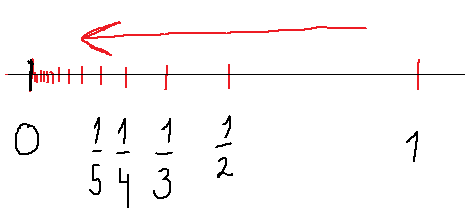
\includegraphics[width=0.4\textwidth]{slike/lim1.png}
\end{figure}

Na enak način predstavimo še naslednja zaporedja in pogledamo, kam se stekajo:
\begin{itemize}
    \item $ \frac{1}{2}, \frac{2}{3}, \frac{3}{4}, \frac{4}{5} \ldots $  (proti 1 z desne)
    \item $ 1, -1, \frac{1}{2}, -\frac{1}{2}, \frac{1}{3}, -\frac{1}{3} \ldots $ (proti 0 z obeh strani)
    \item $ \frac{1}{2}, -\frac{1}{2}, \frac{2}{3}, -\frac{2}{3} \ldots $ (navzven iz 0 proti -1 in 1)
\end{itemize}

\begin{figure}[h]
    \centering
    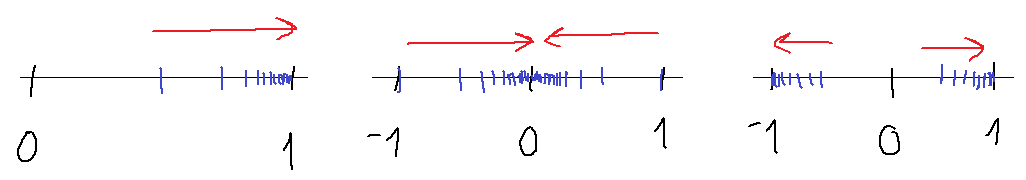
\includegraphics[width=\textwidth]{slike/lim2.png}
\end{figure}

Ta števila, proti katerim grejo členi, bomo imenovali \textbf{stekališča}.

Definirajmo \textbf{okolico točke a na premici} = odprt interval oblike $ (a - \epsilon, a + \epsilon) $, kjer je $\epsilon$ poljubno realno število $ > 0 $.

\begin{figure}[h]
    \centering
    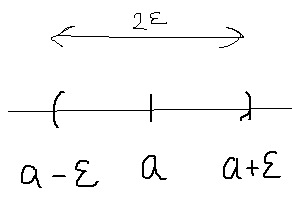
\includegraphics[width=0.3\textwidth]{slike/e_okolica.png}
\end{figure}

\textbf{Stekališče} je število, v čigar okolici \didopomba{poljubno majhnem intervalu okoli tega števila} je neskončno členov zaporedja \didopomba{vsi štirje prejšnji primeri imajo eno ali 2 stekališči}.

\begin{figure}[h]
    \centering
    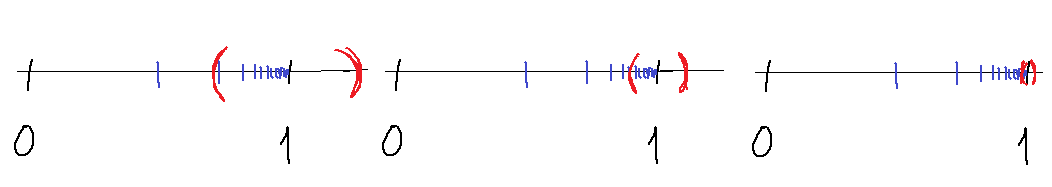
\includegraphics[width=\textwidth]{slike/e_okolica_primer.png}
\end{figure}

\newpage

Opomba: končno zaporedje ne more imeti stekališča \ldots

Če je $ a $ edino stekališče zaporedja $ a_n $ in je zunaj njegove okolice vedno končno členov zaporedja, ga imenujemo \textbf{limita zaporedja}. Pišemo 

$$ a = \lim_{n \rightarrow \infty} a_n .$$

\didopomba{Če imamo samo pogoj, da je $ a $ edino stekališče, to ni nujno limita, npr. zaporedje $ 0, 1, 0, 2, 0, 3, 0 \ldots $ ali $ 1, 2, 1/2, 3, 1/3, 4, 1/4, 5 \ldots $}

Opomba: Zaporedje, ki ima limito, je \textbf{konvergentno} (se nagiba). Zaporedje, ki nima limite, imenujemo \textbf{divergentno} (se ne nagiba nikamor).

Lastnosti \didopomba{Lahko konkreten primer.}:
\begin{itemize}
    \item $ lim_{n \rightarrow \infty} c = c $
    \item $ lim_{n \rightarrow \infty} (a_n \pm b_n) = lim_{n \rightarrow \infty} a_n \pm lim_{n \rightarrow \infty} b_n $
    \item $ lim_{n \rightarrow \infty} (a_n \cdot b_n) = lim_{n \rightarrow \infty} a_n \cdot lim_{n \rightarrow \infty} b_n $
        \subitem poseben primer množenja s konstantnim zaporedjem $ k $ \didopomba{logično}: $ lim_{n \rightarrow \infty} (k \cdot b_n) = k \cdot lim_{n \rightarrow \infty} b_n $
    \item $ lim_{n \rightarrow \infty} \frac{a_n}{b_n} = \frac{lim_{n \rightarrow \infty} a_n}{lim_{n \rightarrow \infty} b_n}; lim_{n \rightarrow \infty} b_n \ne 0 $
\end{itemize}

\vaje{
Vaje \didopomba{stopnjuješ uporabo zgornjih lastnosti}:
\begin{itemize}
    \item $ lim_{n \rightarrow \infty} \frac{3n + 2}{n - 1} $ (deljenje z $n$, še nekaj podobnih)
    \item $ a_n = \frac{2n}{n+1} $. Zapiši prvih pet členov in izračunaj limito. Kateri členi (za katere $n$) ležijo zunaj okolice limite s polmerom 0,4? ($ |2 - \frac{2n}{n+1}| \geq \frac{4}{10} $)
    \item racionalizacija: $ lim_{n \rightarrow \infty} (\sqrt{n+1} - \sqrt{n-1}) $
    \item $ lim_{n \rightarrow \infty} (1 + \frac{1}{n})^n = e $ (s kalkulatorjem prvih nekaj členov. Povemo, da pač to je to. Uporabimo na nadaljnih primerih npr. $ lim_{n \rightarrow \infty} (1 + \frac{4}{3n})^{5n}) $
\end{itemize}
}
 
\end{priprava}